% DO NOT COMPILE THIS FILE DIRECTLY!
% This is included by the other .tex files.

\begin{frame}
\titlepage
\end{frame}

\begin{frame}
  \frametitle{What happened in the past 6 months?}
  \begin{itemize}
    \item {\bf 13} new MISP {\bf releases} - on track for ~2 / month
    \item Over {\bf 2000 commits} for the core alone from {\bf 34 contributors}
    \item Progress on a massive rework that is underways
    \item Before we get to the highlights...
  \end{itemize}
\end{frame}

\begin{frame}
  \frametitle{Standardisation for open source formats}
  \begin{itemize}
    \item \url{https://www.misp-standard.org}
    \item Standardising the {\bf MISP related} and {\bf other open source} formats
    \item We want a vehicle for publishing standards {\bf without giving up control}
    \item Let us know if you would like to be listed!
  \end{itemize}
\end{frame}

\begin{frame}
  \frametitle{Steady growth in efforts to share refined information}
  \begin{itemize}
    \item Both on a {\bf data} and a {\bf context} level
    \item Growth in the {\bf community's} and {\bf tooling's} maturity
    \item {\bf ATT\&CK}'s quick adoption is partially to blame for recent surge
    \item Also a side effect of MISP becoming a sharing tool for completely {\bf different domains}
  \end{itemize}
\end{frame}

\begin{frame}
  \frametitle{Object relations}
  \begin{center}
    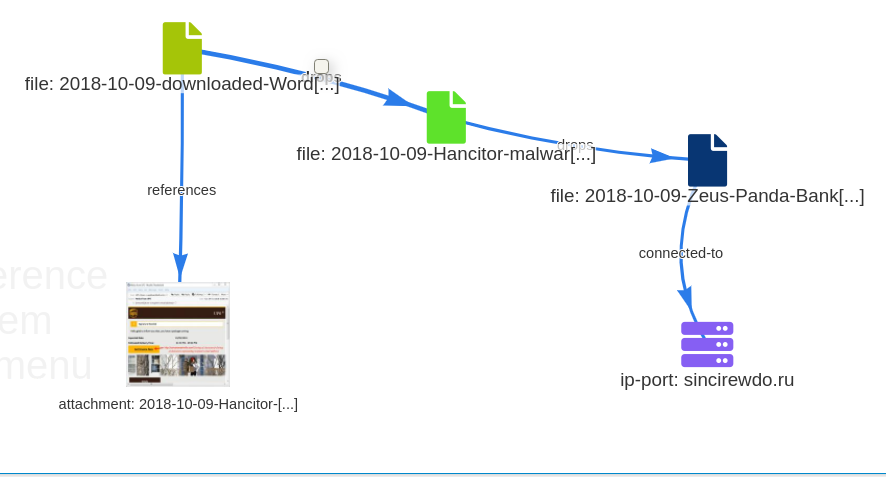
\includegraphics[width=1.0\linewidth]{story.png}
  \end{center}
\end{frame}


\begin{frame}
  \frametitle{ATT\&CK}
  \begin{center}
    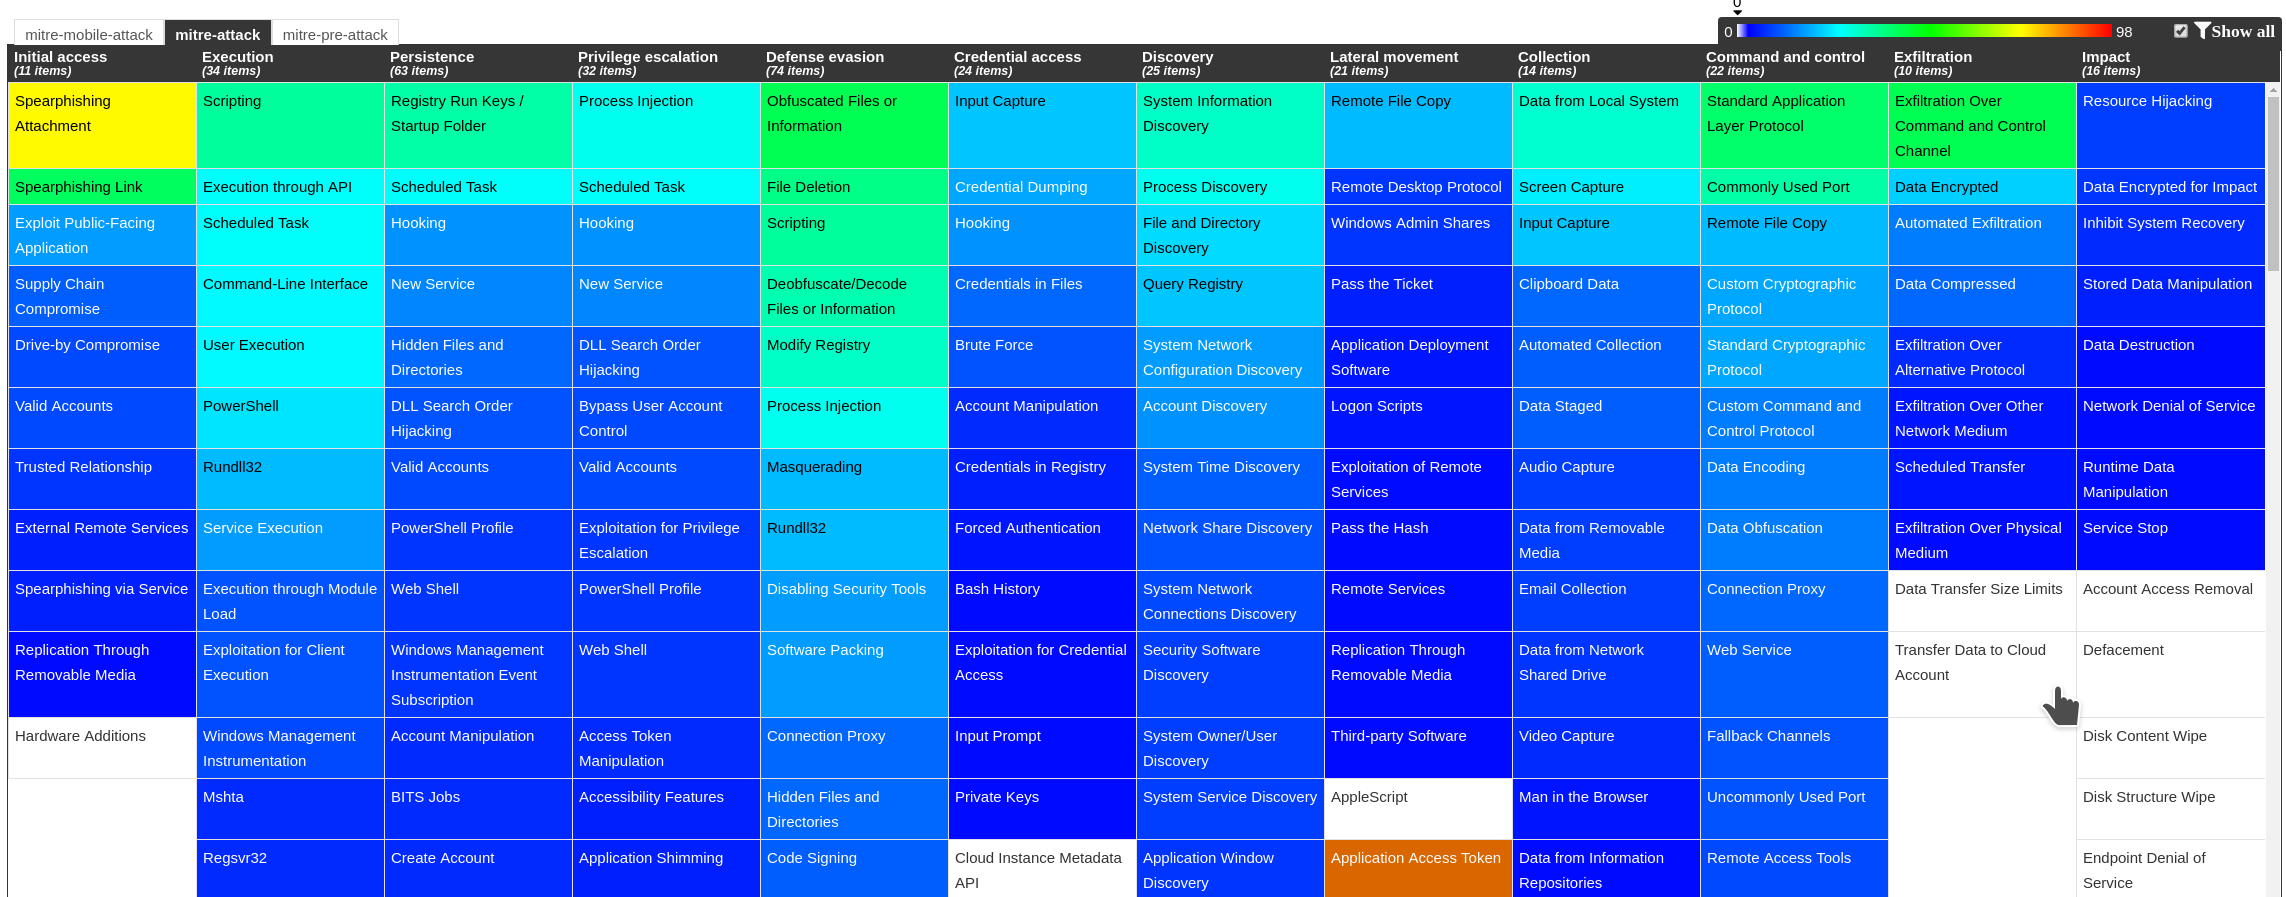
\includegraphics[width=1.0\linewidth]{attack.png}
  \end{center}
\end{frame}

\begin{frame}
  \frametitle{ATT\&CK like matrices}
  \begin{center}
    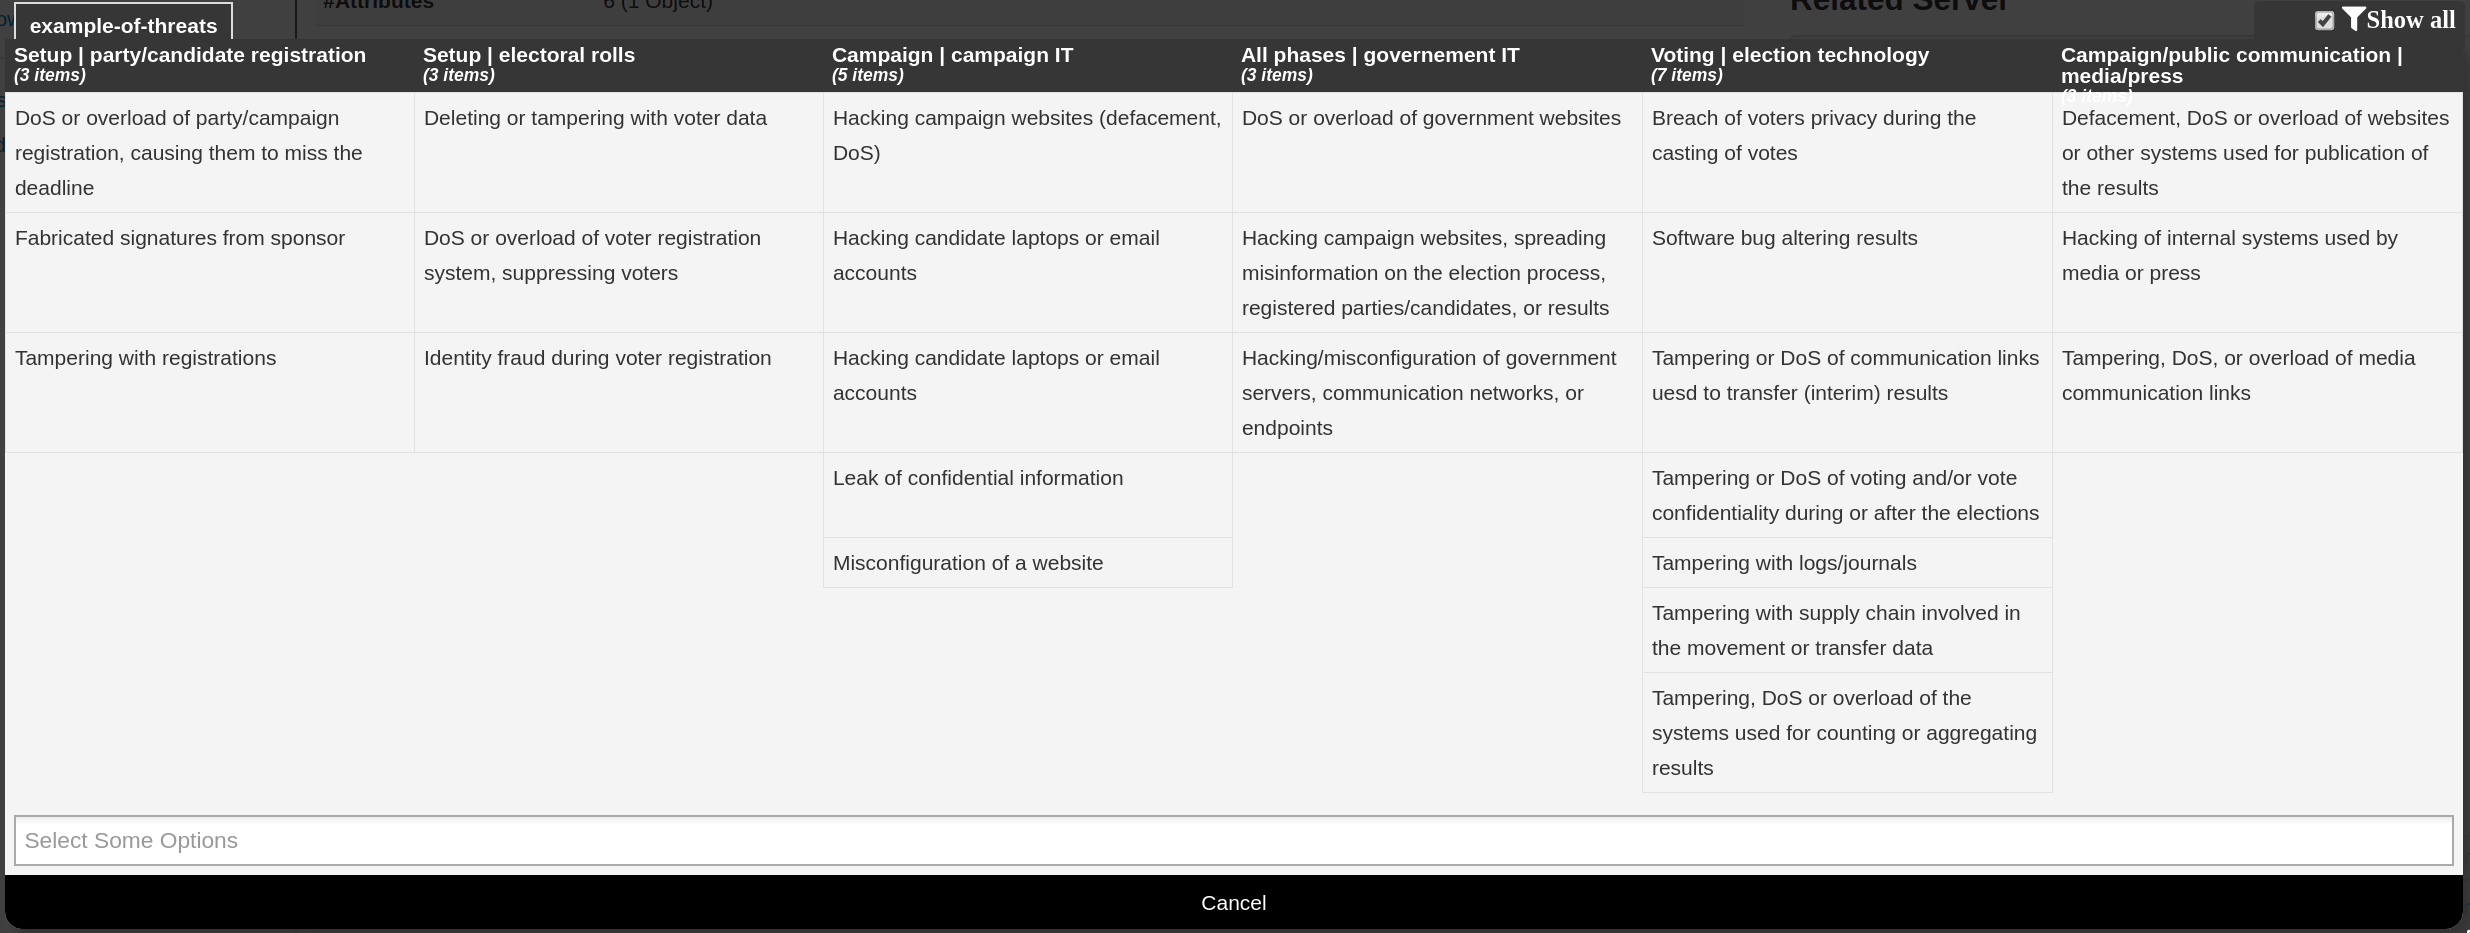
\includegraphics[width=1.0\linewidth]{attack_like.png}
  \end{center}
\end{frame}

\begin{frame}
  \frametitle{Community management}
  \begin{itemize}
    \item Sectorial, regional, topical groupings becoming more organised
    \item Inherently more difficult to find the right communities
    \item We're starting to build an opt-in {\bf community registry}
    \item Still very early days, but let us know if you would like to {\bf announce yourselves}!
  \end{itemize}
\end{frame}


\begin{frame}
  \frametitle{Community request}
  \begin{center}
    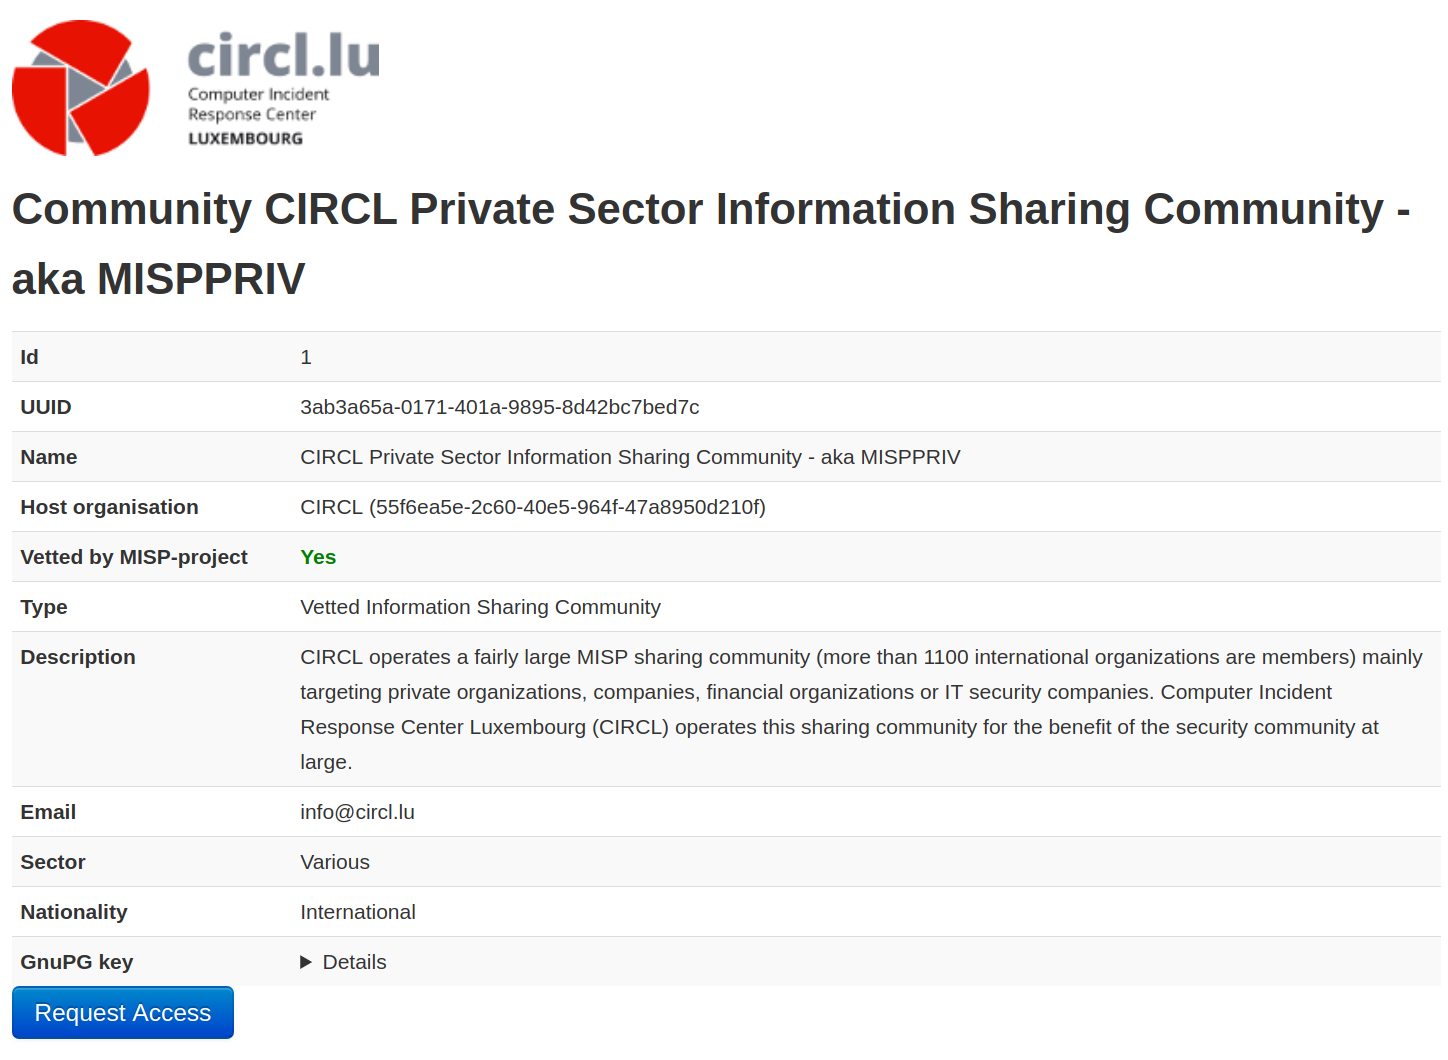
\includegraphics[width=1.0\linewidth]{community_request.png}
  \end{center}
\end{frame}

\begin{frame}
  \frametitle{Sightings improved}
  \begin{itemize}
    \item More organisations involved in the feedback-loop of reporting back sightings
    \item Sighting synchronisation improved
    \item Alternate sighting back-end for heavy, bulk sightings
    \item SightingDB, open source, developed by Devo
    \item Experimental for now, but fully functional.
    \item SightingDB standard for alternate implementations via misp-standard.org
  \end{itemize}
\end{frame}

\begin{frame}
  \frametitle{Various improvements to taxonomies}
  \begin{itemize}
    \item Tag exclusivity allows for taxonomies with inherent rules
    \begin{itemize}
      \item For example: It makes no sense to have multiple TLP tags on an event
      \item You can also restrict on a predicate level
    \end{itemize}
    \item Require taxonomies to be set
    \begin{itemize}
      \item Certain taxonomies can be set as requirements for publishing in a community
      \item Example: No TLP/PAP? No right to publish.
    \end{itemize}
  \end{itemize}
\end{frame}

\begin{frame}
  \frametitle{Alerting rules}
  \begin{itemize}
    \item First steps for our user settings system
    \item Customise the rules that decide what you want to get alerted on
  \end{itemize}
  \begin{center}
    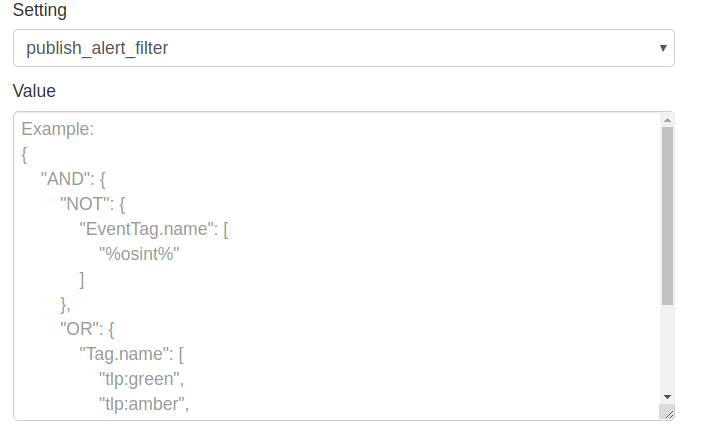
\includegraphics[width=0.8\linewidth]{publish_alert.png}
  \end{center}
\end{frame}

\begin{frame}
  \frametitle{Decaying of indicators}
  \begin{itemize}
    \item MISP has a powerful toolbox that allows users to filter their dataset based on their needs
    \item We were still missing a way to use all of these systems in combination to decay indicators
    \item Move the decision making \textbf{from complex filter options to} complex \textbf{decay models}
    \item Decay models would take into account various \textbf{taxonomies}, \textbf{sightings}, the \textbf{type} of each indicator \textbf{Sightings} and \textbf{Creation date}
    \item The first iteration of what we have in MISP now took:
    \begin{itemize}
       \item 2 years of research
       \item 3 published research papers
       \item A lot of prototyping
    \end{itemize}
  \end{itemize}
\end{frame}

\begin{frame}
    \frametitle{Scoring Indicators: Our solution}
    $$ \texttt{score}(\texttt{\tiny Attribute}) = \texttt{base\_score}(\texttt{\tiny Attribute, Model}) \;\;\bullet\;\; \texttt{decay}(\texttt{\tiny Model, time}) $$
    Where,\vspace{0.5cm}
    \begin{itemize}
        \item \texttt{score} $ \in [0, 100] $
        \item \texttt{base\_score} $ \in [0, 100] $
        \item \texttt{decay} is a function defined by model's parameters controlling decay speed
        \item \texttt{Attribute} Contains \textit{Attribute}'s values and metadata {\scriptsize (\textit{Taxonomies}, \textit{Galaxies}, ...)}
        \item \texttt{Model} Contains the \textit{Model}'s configuration
    \end{itemize}
\end{frame}

\begin{frame}
    \frametitle{Implementation in MISP: \texttt{Event/view}}
    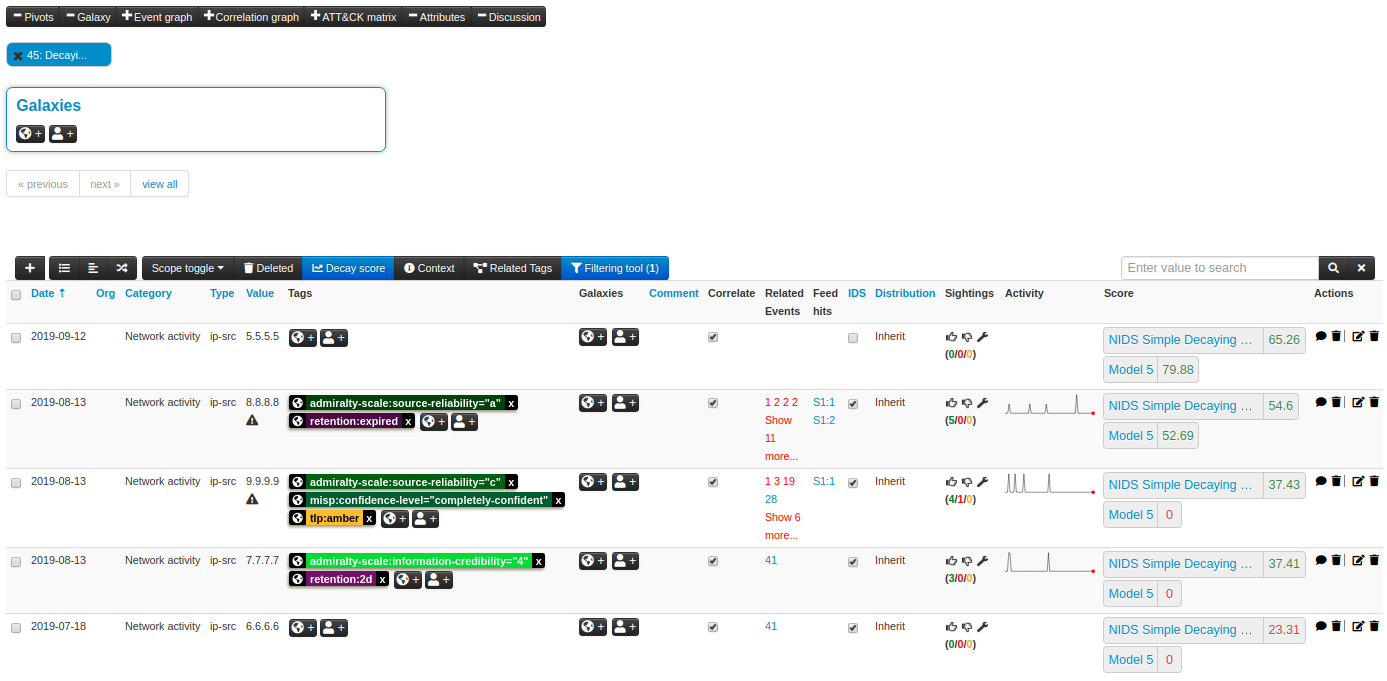
\includegraphics[width=1.00\linewidth]{decaying-event.png}
    \begin{itemize}
        \item \texttt{Decay score} toggle button
        \begin{itemize}
            \item Shows Score for each \textit{Models} associated to the \textit{Attribute} type
        \end{itemize}
    \end{itemize}
\end{frame}

\begin{frame}[fragile]
    \frametitle{Implementation in MISP: API result}
    \texttt{/attributes/restSearch}
    \begin{lstlisting}
"Attribute": [
  {
    "category": "Network activity",
    "type": "ip-src",
    "to_ids": true,
    "timestamp": "1565703507",
    [...]
    "value": "8.8.8.8",
    "decay_score": [
      {
        "score": 54.475223849544456,
        "decayed": false,
        "DecayingModel": {
          "id": "85",
          "name": "NIDS Simple Decaying Model"
        }
      }
    ],
[...]
    \end{lstlisting}
\end{frame}


\begin{frame}
    \frametitle{Implementation in MISP: Index}
    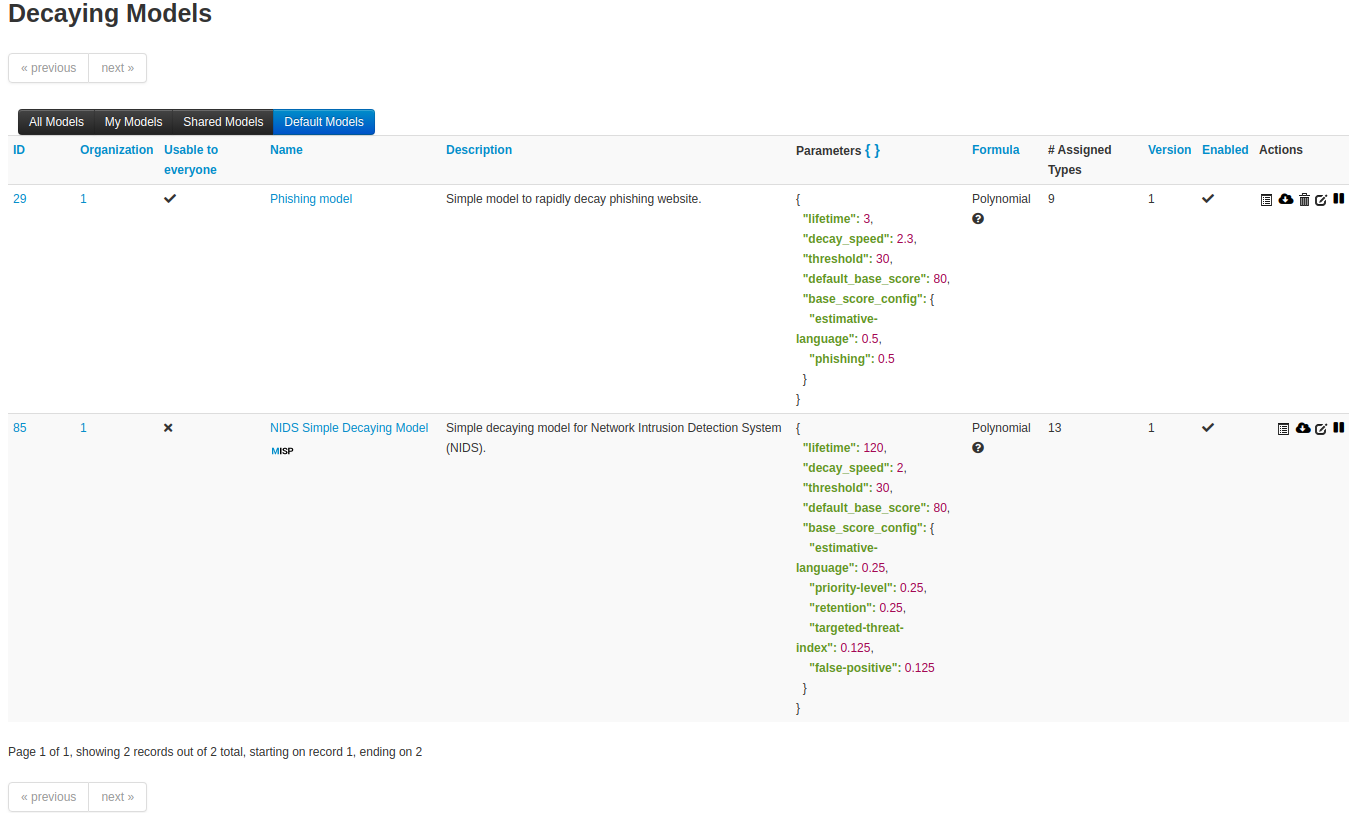
\includegraphics[width=1.00\linewidth]{decaying-index.png}
    View, update, add, create, delete, enable, export, import
\end{frame}

\begin{frame}
    \frametitle{Implementation in MISP: Fine tuning tool}
    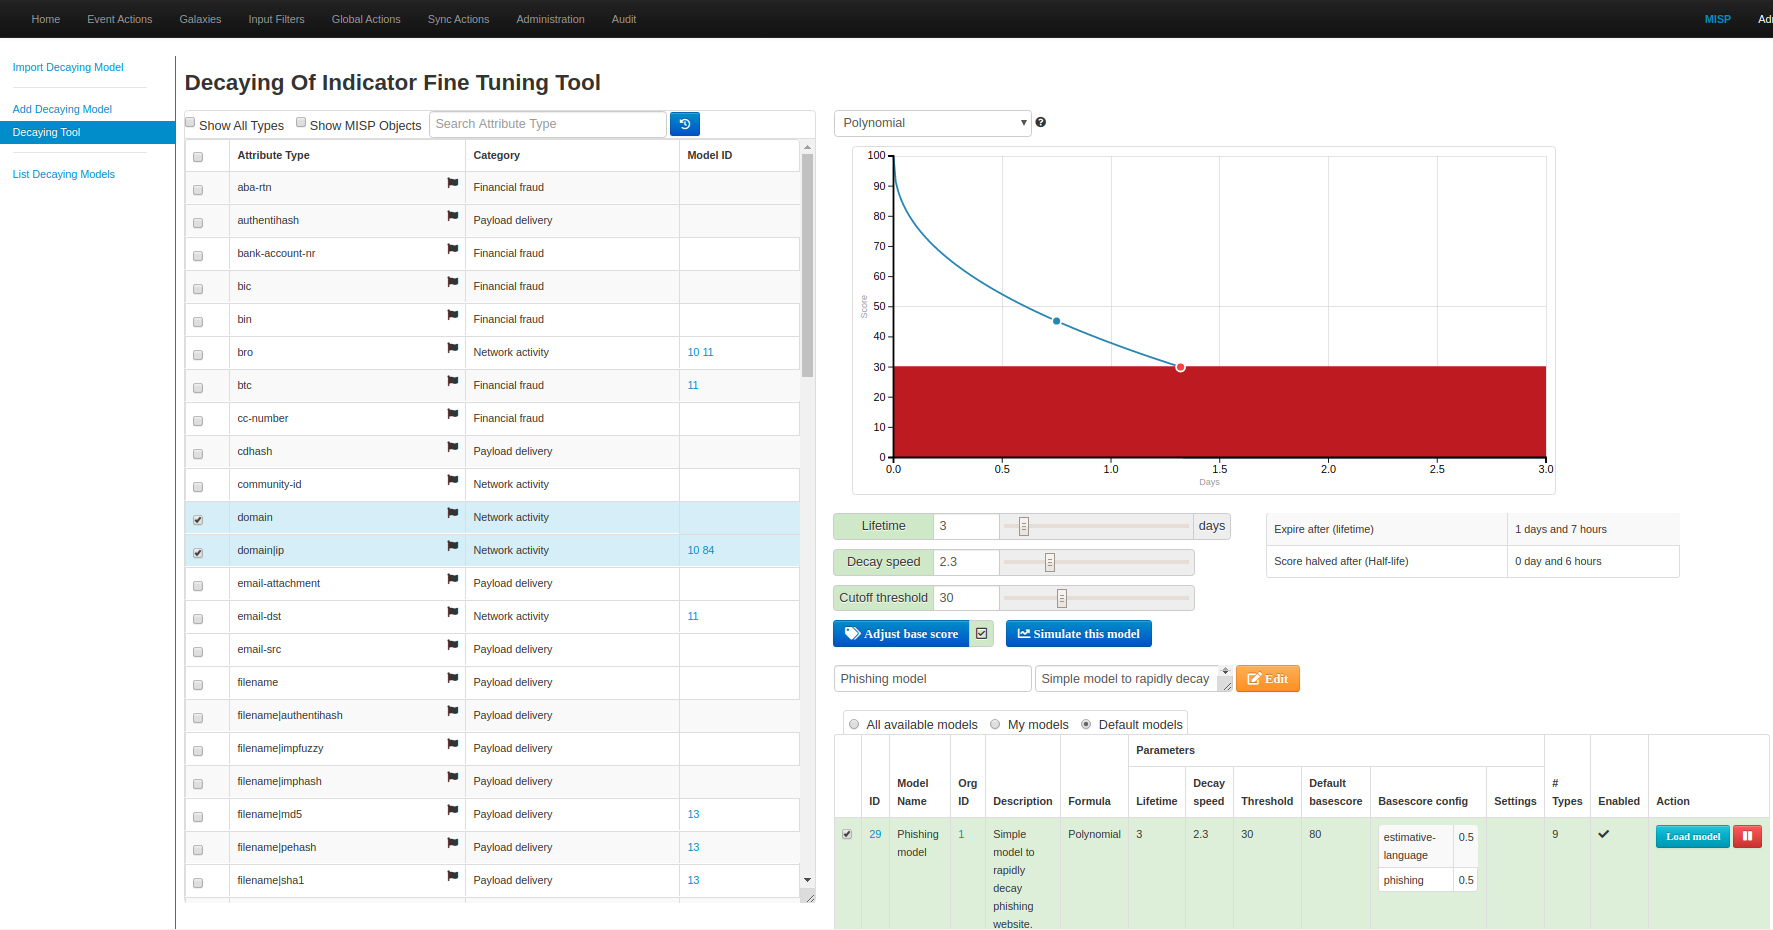
\includegraphics[width=1.00\linewidth]{decaying-tool.png}
    Create, modify, visualise, perform mapping
\end{frame}

\begin{frame}
    \frametitle{Implementation in MISP: \texttt{base\_score} tool}
    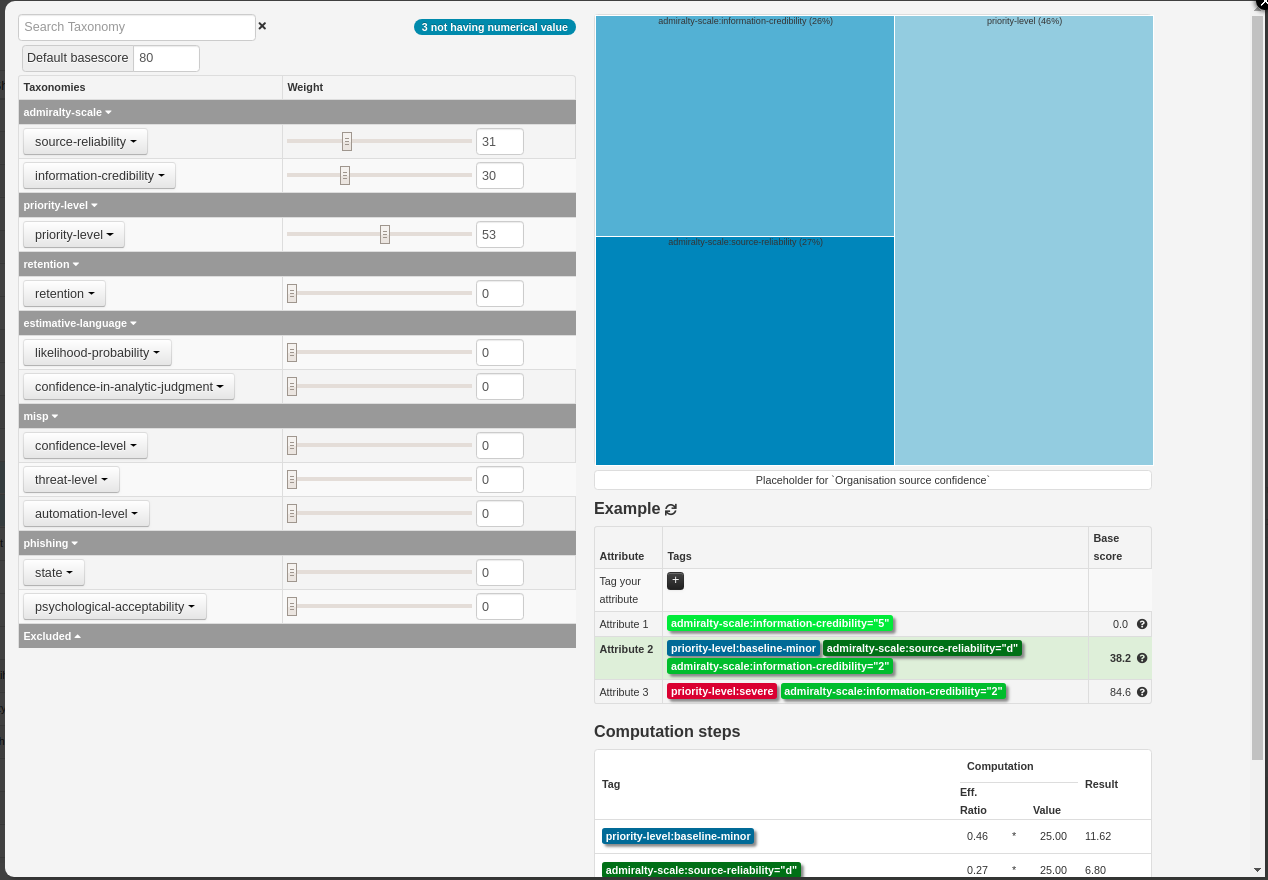
\includegraphics[width=1.00\linewidth]{decaying-basescore.png}
    Adjust Taxonomies relative weights
\end{frame}

\begin{frame}
    \frametitle{Implementation in MISP: simulation tool}
    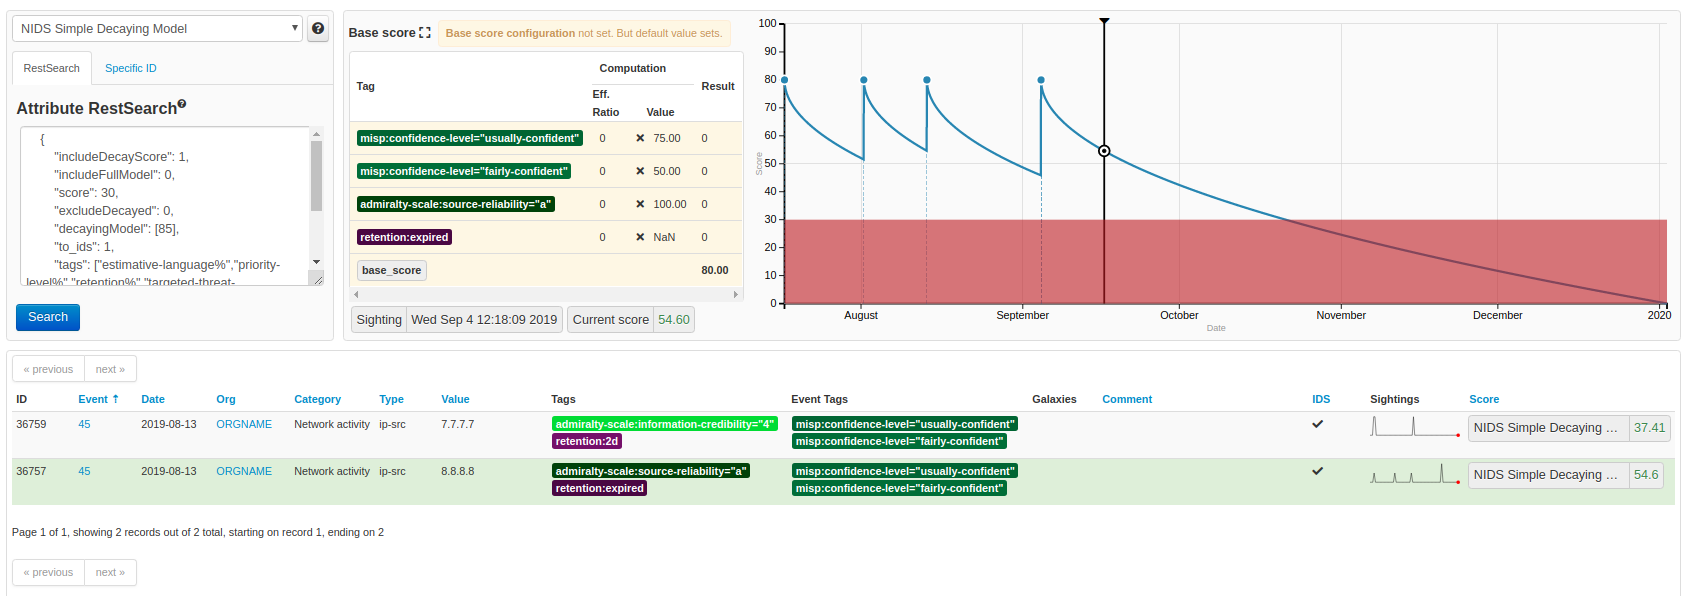
\includegraphics[width=1.00\linewidth]{decaying-simulation.png}
    Simulate \textit{Attributes} with different \textit{Models}
\end{frame}

\begin{frame}[fragile]
    \frametitle{Implementation in MISP: API query body}
    \texttt{/attributes/restSearch}
    \begin{lstlisting}
{
    "includeDecayScore": 1,
    "includeFullModel": 0,
    "excludeDecayed": 0,
    "decayingModel": [85],
    "modelOverrides": {
        "threshold": 30
    }
    "score": 30,
}
    \end{lstlisting}
\end{frame}

\begin{frame}
  \frametitle{Where do we go from here?}
  \begin{itemize}
    \item Massive list of features/todos
    \item Most immediate ones we're working on:
    \begin{itemize}
      \item {\bf Community management} via a new, related tool called {\bf Cerebrate} coming 2020
      \item {\bf Custom galaxies}, editing in MISP directly
      \item Massive {\bf rework} moving MISP to a more modern version of the framework
      \item Internal refactor / deprecation of old baggage
      \item {\bf New UI}
    \end{itemize}
\end{frame}


\begin{frame}
  \frametitle{Get in touch if you have any questions}
  \begin{itemize}
    \item Contact CIRCL
    \begin{itemize}
      \item info@circl.lu
      \item \url{https://twitter.com/circl_lu}
      \item \url{https://www.circl.lu/}
    \end{itemize}
    \item Contact MISPProject 
    \begin{itemize}
      \item \url{https://github.com/MISP}
      \item \url{https://gitter.im/MISP/MISP}
      \item \url{https://twitter.com/MISPProject}
    \end{itemize}
    \item Poke me directly
    \begin{itemize}
      \item \url{https://twitter.com/iglocska}
    \end{itemize}
  \end{itemize}
\end{frame}
